\section{Konklusion}
\begin{frame}{Konklusion}
\begin{itemize}
	\item How have the upper and lower bounds of the Rubik's Cube progressed and how have they been proven?
	\begin{itemize}
		\item Den \o{}vre gr\ae{}nse er bevist med Rokicki's set solver.
		\item Den nedre gr\ae{}nse bevist ved test.
	\end{itemize}
\end{itemize}
\begin{figure}
	\centering
		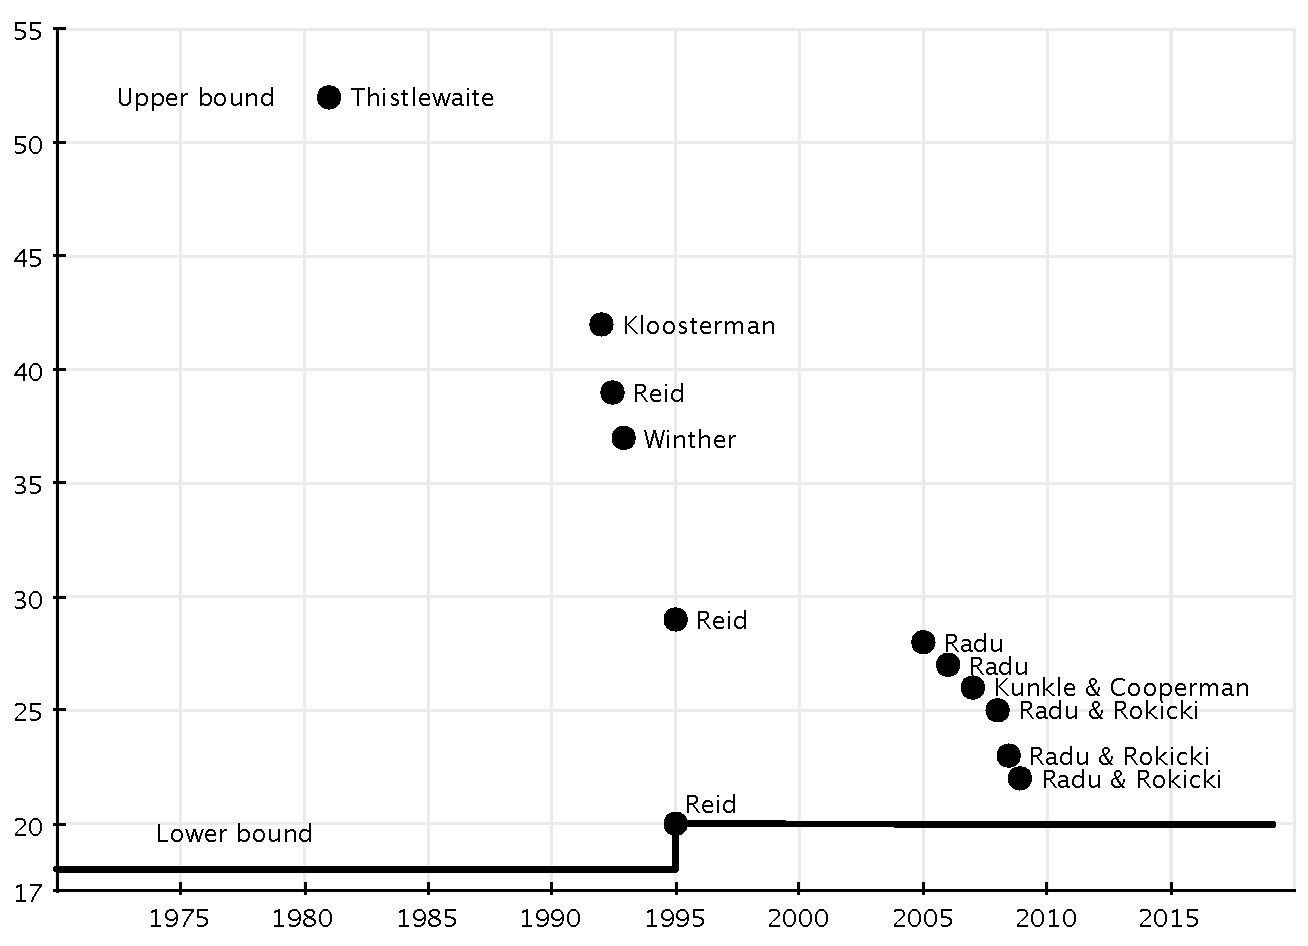
\includegraphics[width=0.6\textwidth]{input/pics/bounds2.pdf}
	%\caption{Udvikling af gr�nserne}
	\label{fig:bounds3}
\end{figure}
\end{frame}

\begin{frame}{Konklusion}
\begin{itemize}
	\item How efficient is Kociemba's optimal solver compared to beginner's algorithm and how can this be tested?
	\begin{itemize}
		\item Twist-wise
		\begin{itemize}
			\item Begynderens bruger i snit 151 tr\ae{}k
			\item Kociemba's bruger altid under 22 tr\ae{}k
		\end{itemize}
		\item Time-wise
		\begin{itemize}
			\item $1,2 \cdot 10^{18}$
		\end{itemize}
		\item Computer tests
	\end{itemize}
\end{itemize}
\end{frame}